\documentclass[border=0.05cm]{standalone}
\usepackage[dvipsnames]{xcolor}
\usepackage{tikz}
\usetikzlibrary {arrows.meta} 
\usepackage[utf8]{inputenc}
\usepackage{anyfontsize}
\usetikzlibrary{decorations.pathreplacing}


\definecolor{myorange}{RGB}{220, 95, 0}
\definecolor{mygreen}{RGB}{144, 210, 109}
\definecolor{myblue}{RGB}{0,159,189}%{80,140,155}
\definecolor{mypink}{RGB}{255, 180, 194}

%\begin{document}
%	\centering
%	\begin{tikzpicture}
%		
%		\node[align=center] at (10cm,6.8cm) {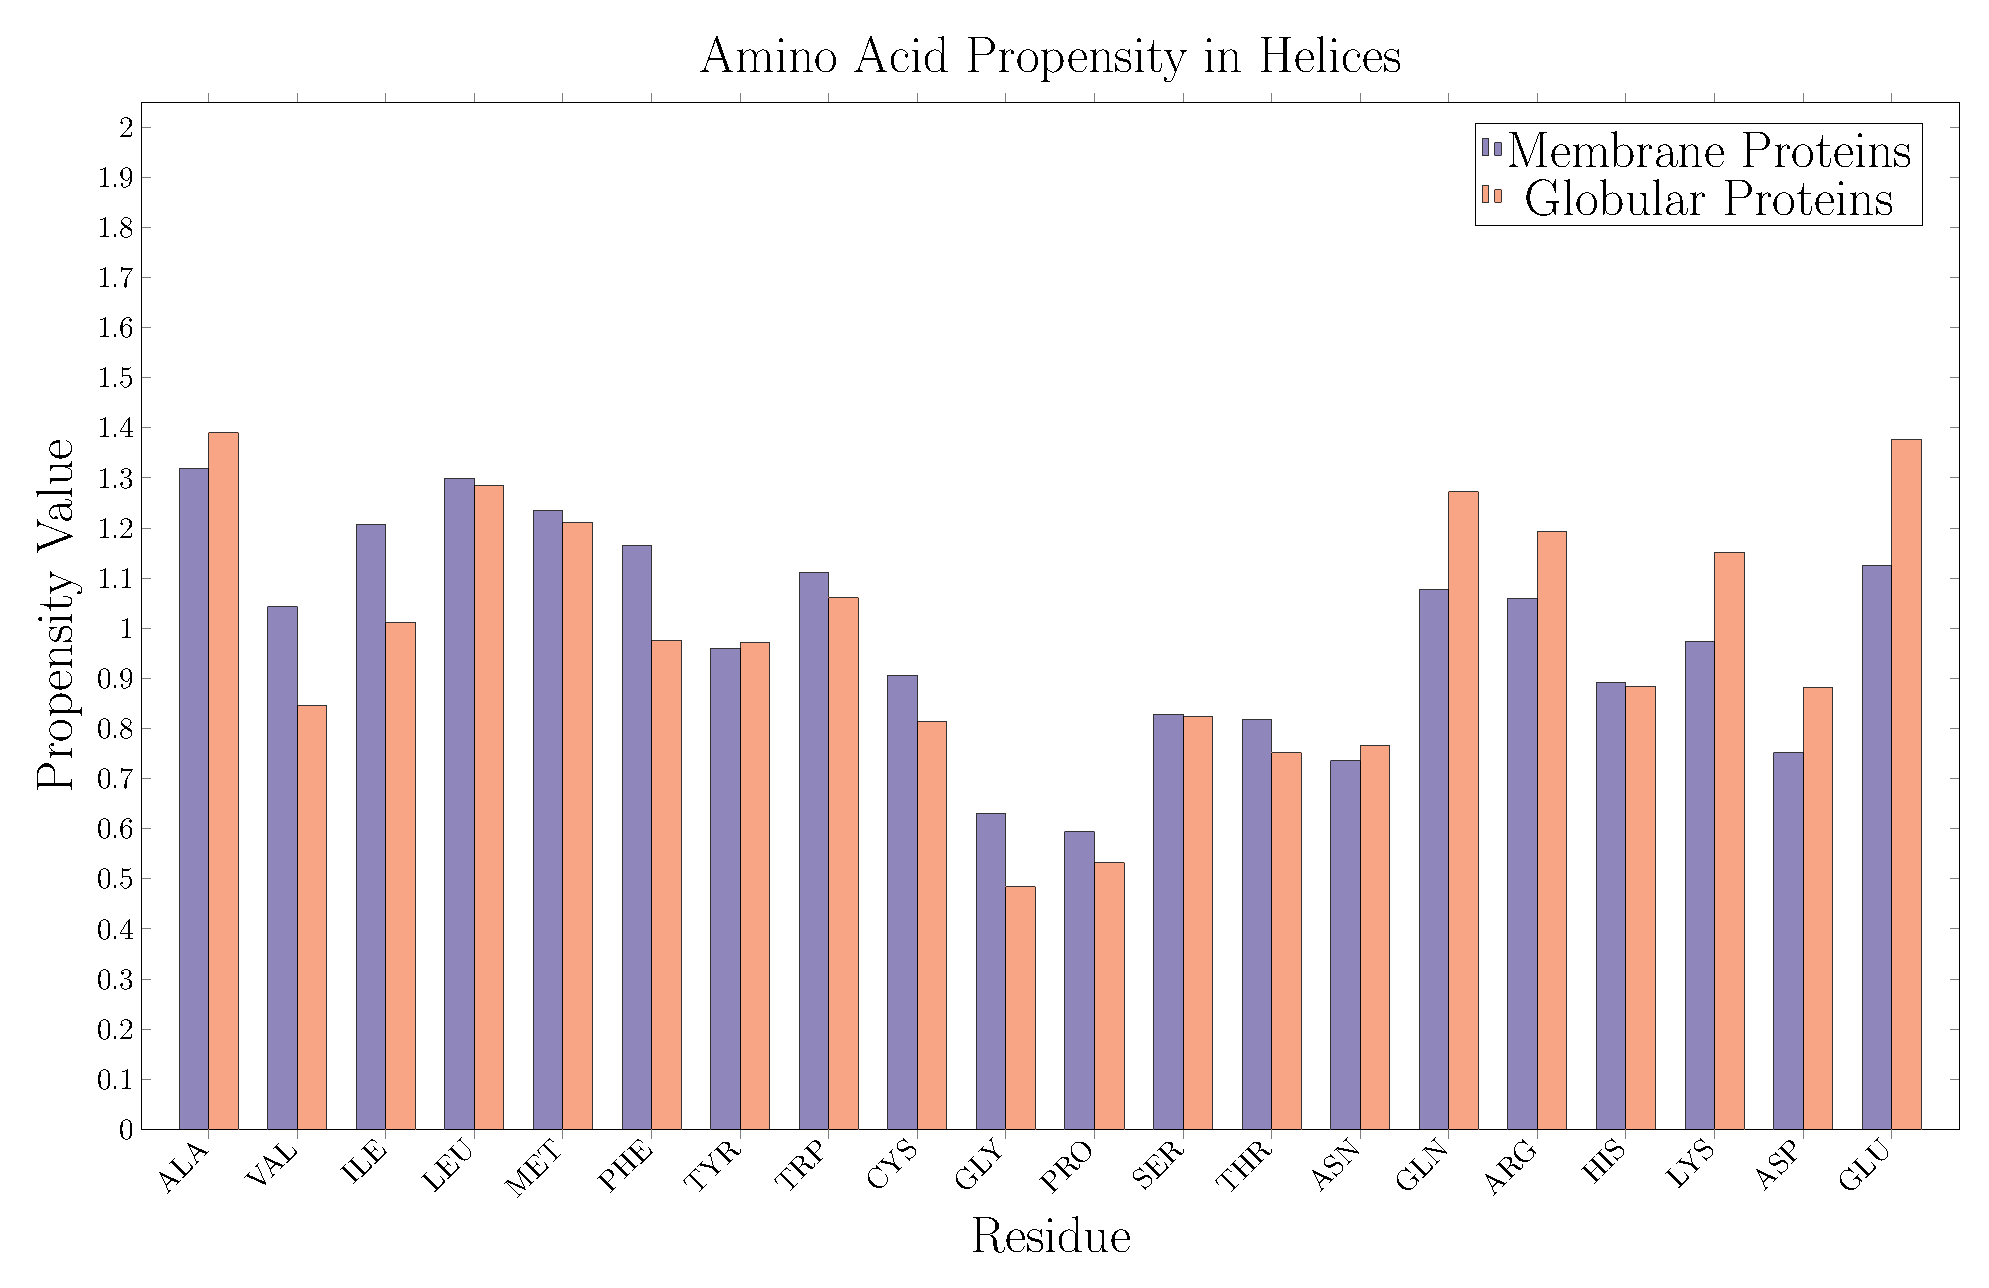
\includegraphics[width=0.025\textheight]{propensity_helices.pdf}};
%		\node[align=center] at (25cm,6.8cm) {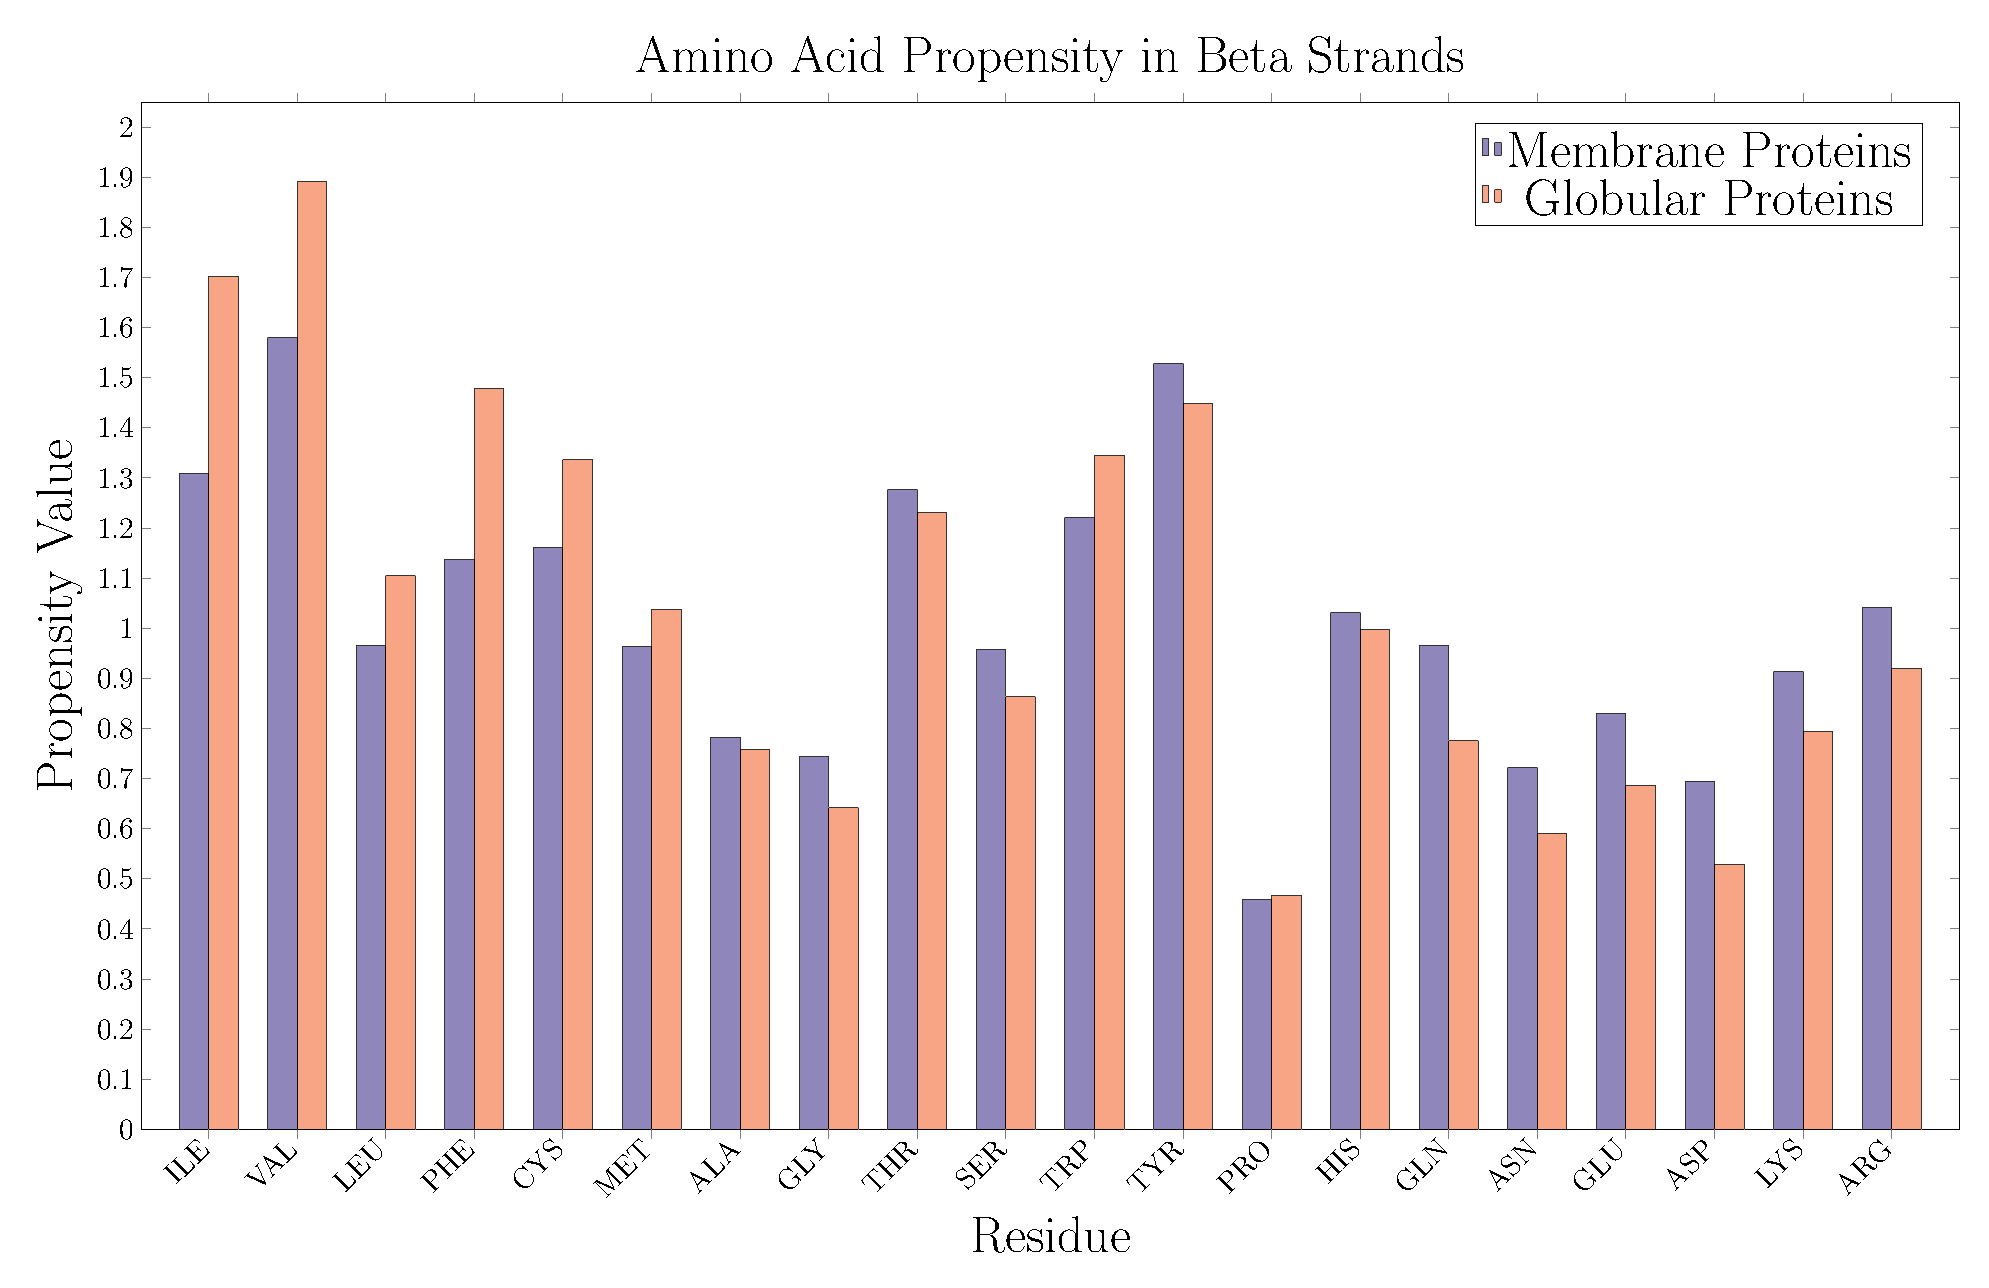
\includegraphics[width=0.025\textheight]{propensity_strands.pdf}};
%		\node[align=center] at (10cm,-6.8cm) {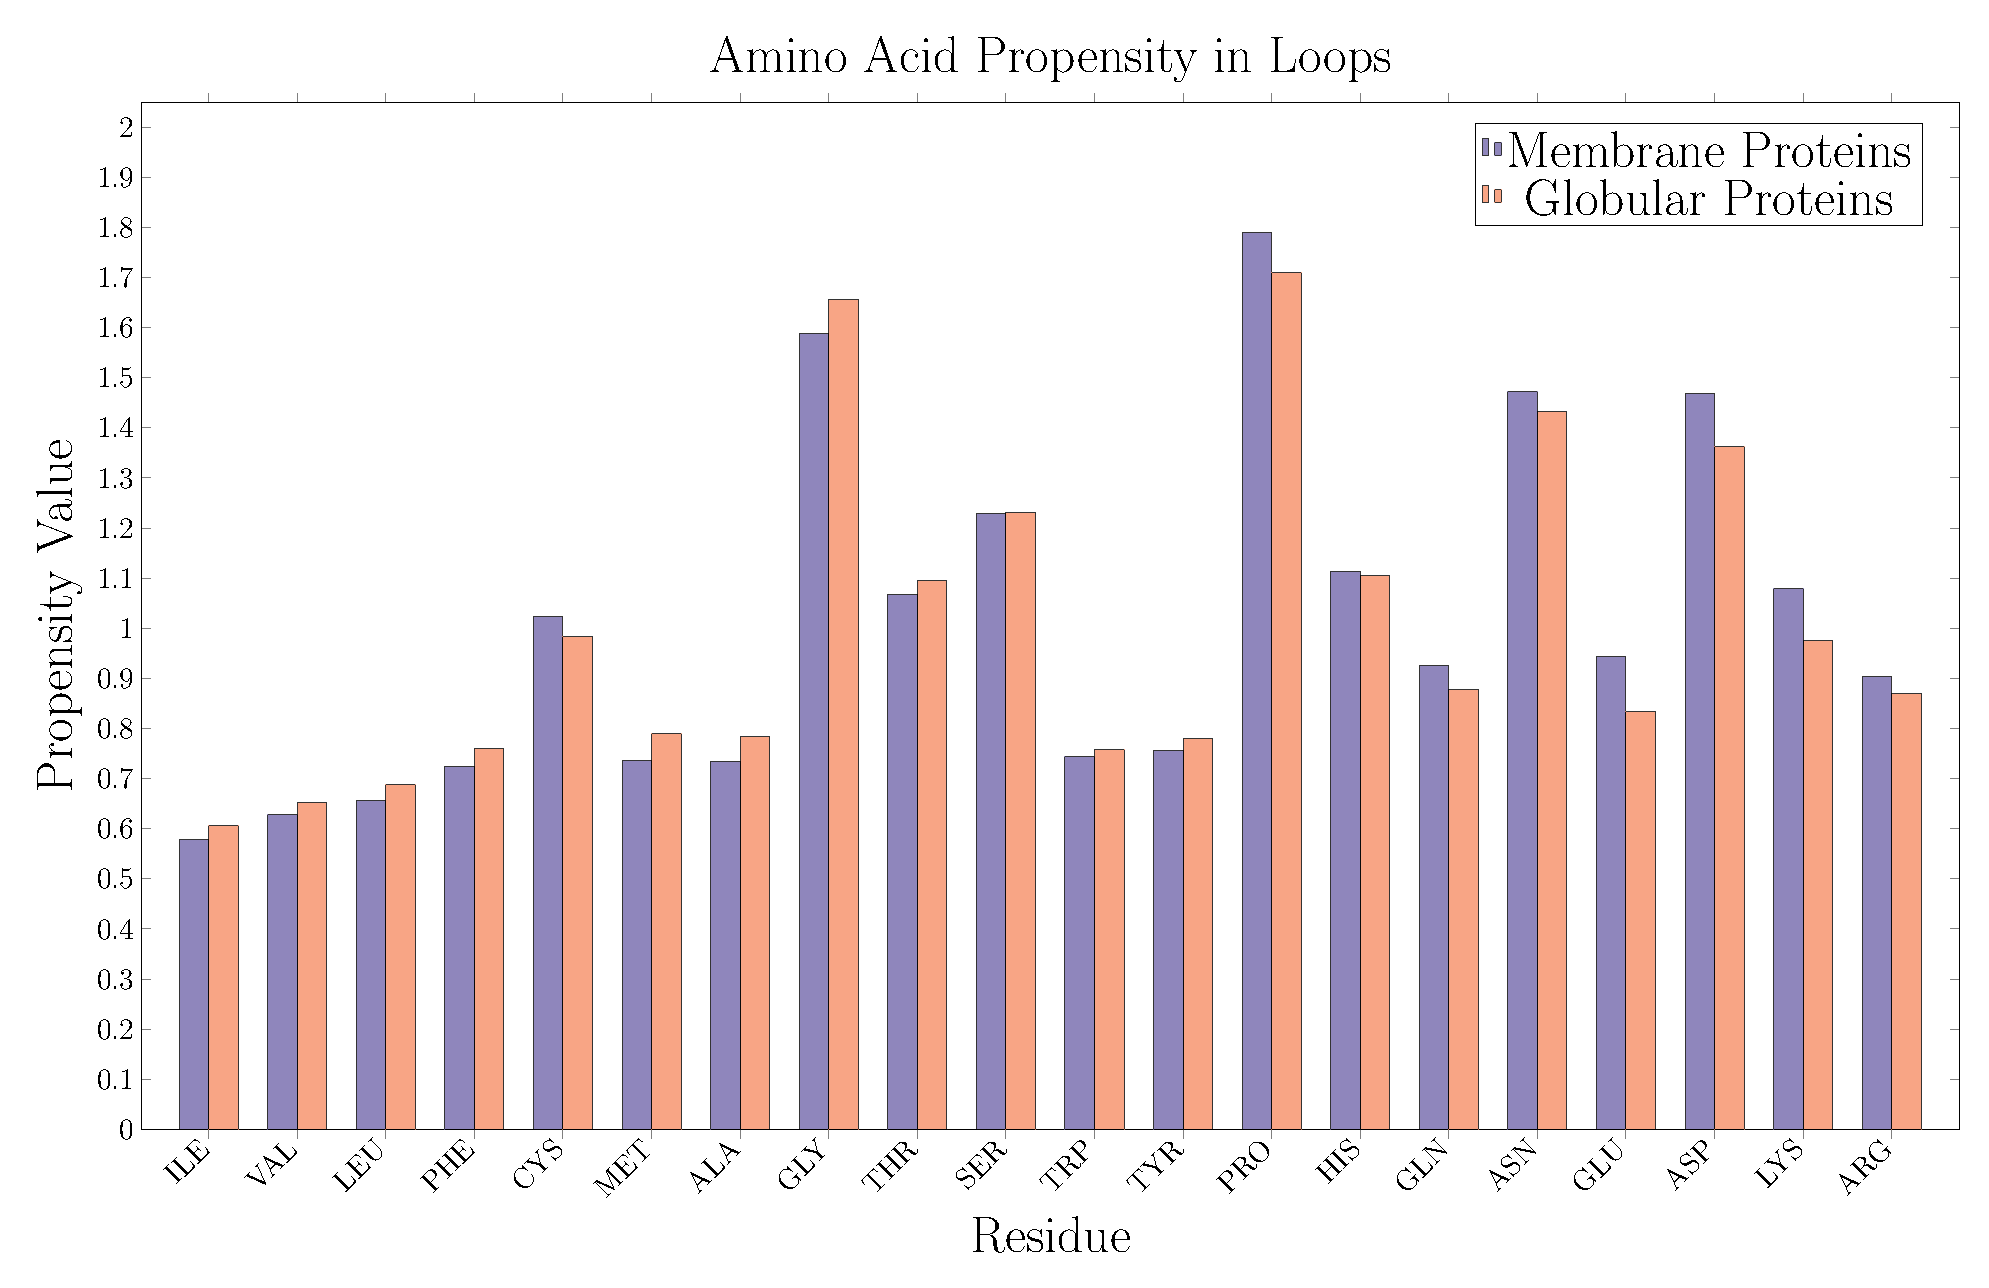
\includegraphics[width=0.025\textheight]{propensity_loops.pdf}};
%		\node[align=center] at (25cm,-7cm) {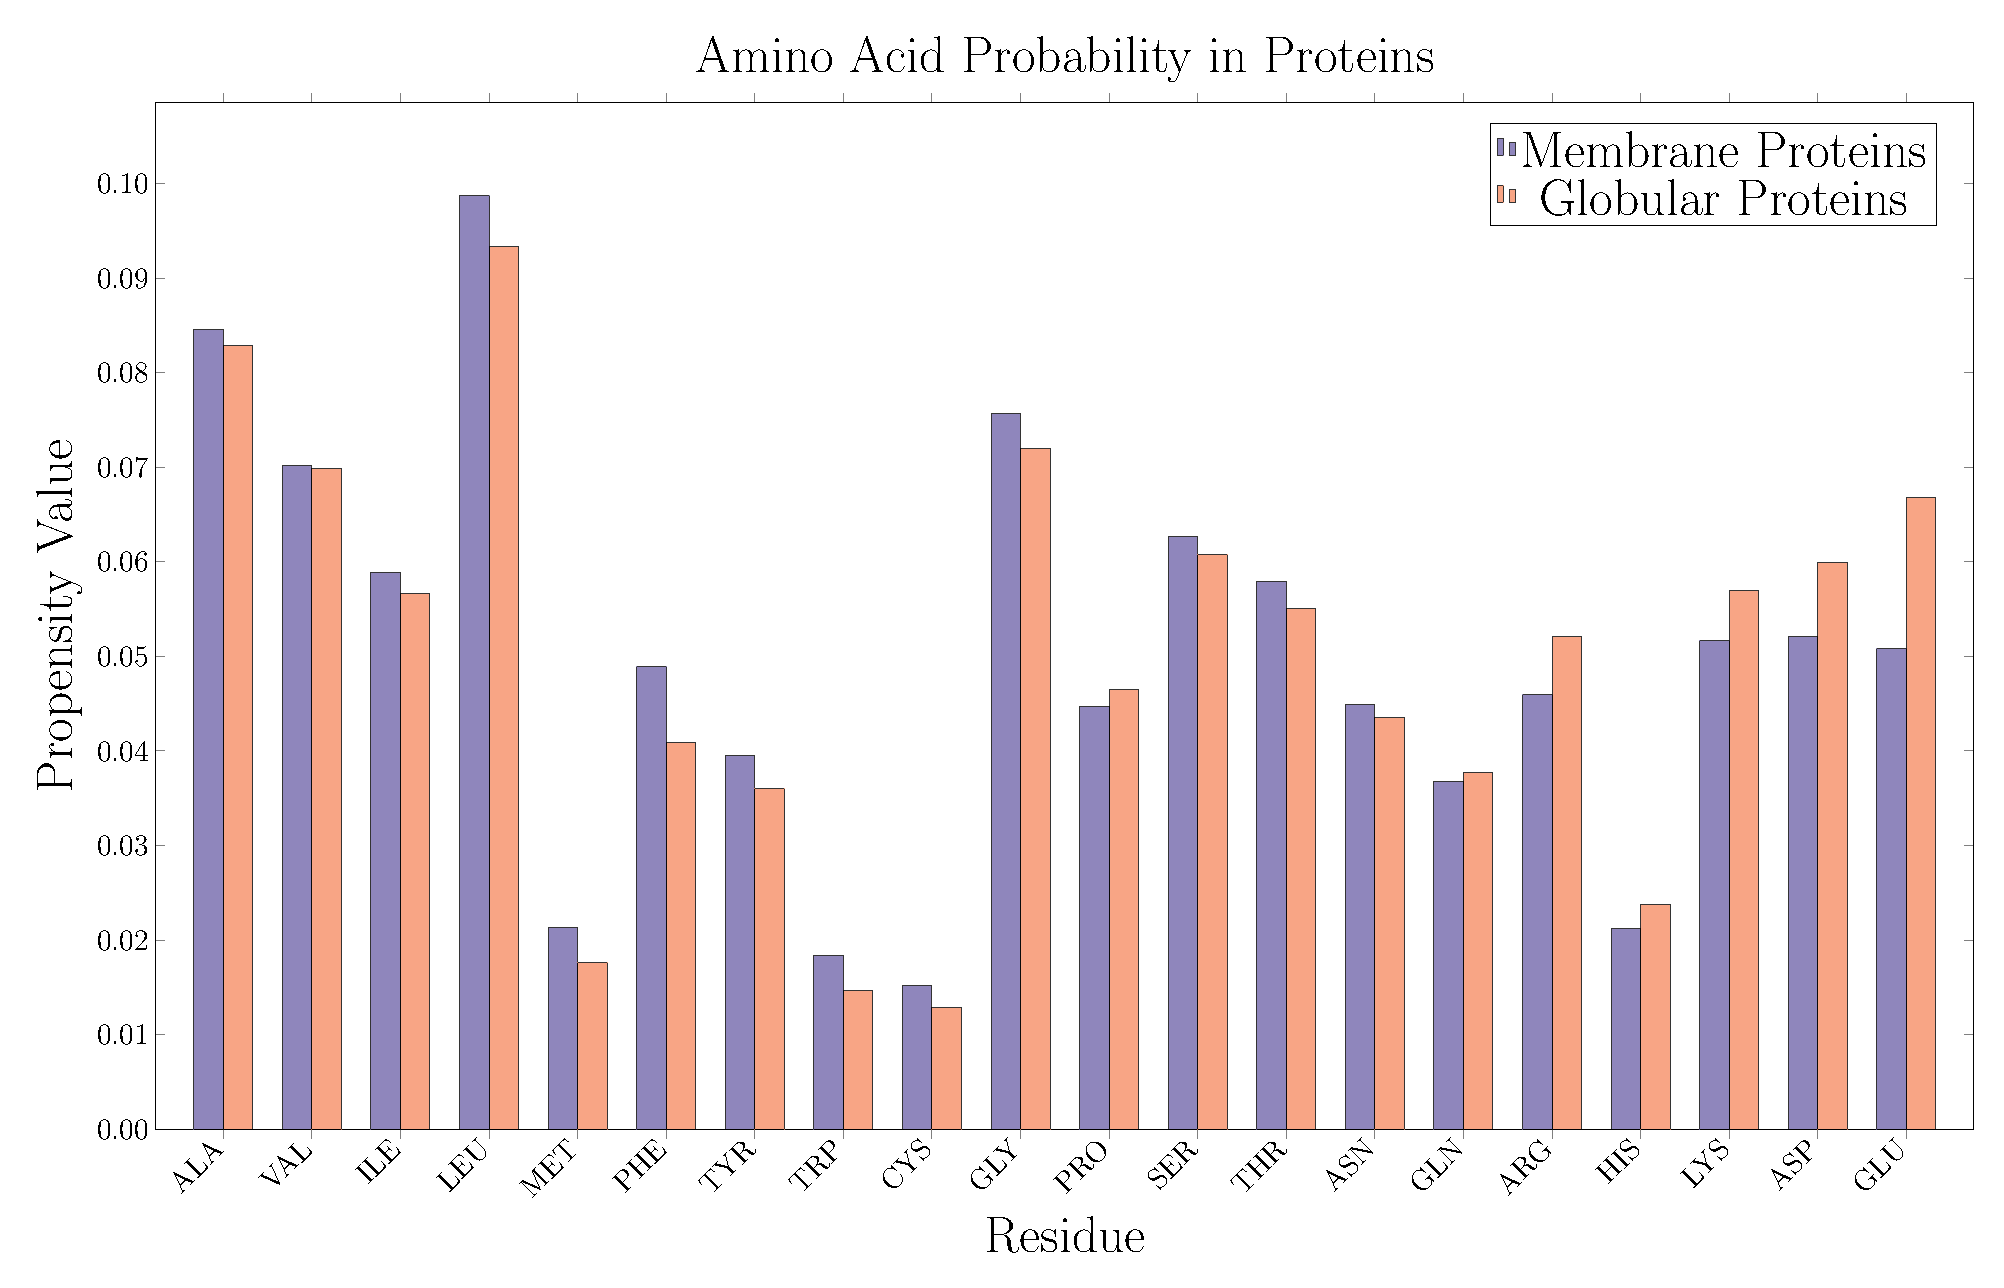
\includegraphics[width=0.025\textheight]{probability_aa.pdf}};
%		
%	\end{tikzpicture}
%\end{document}  

\begin{document}
	\centering
	\begin{tikzpicture}
			
			\node[align=center] at (10cm,5.cm) {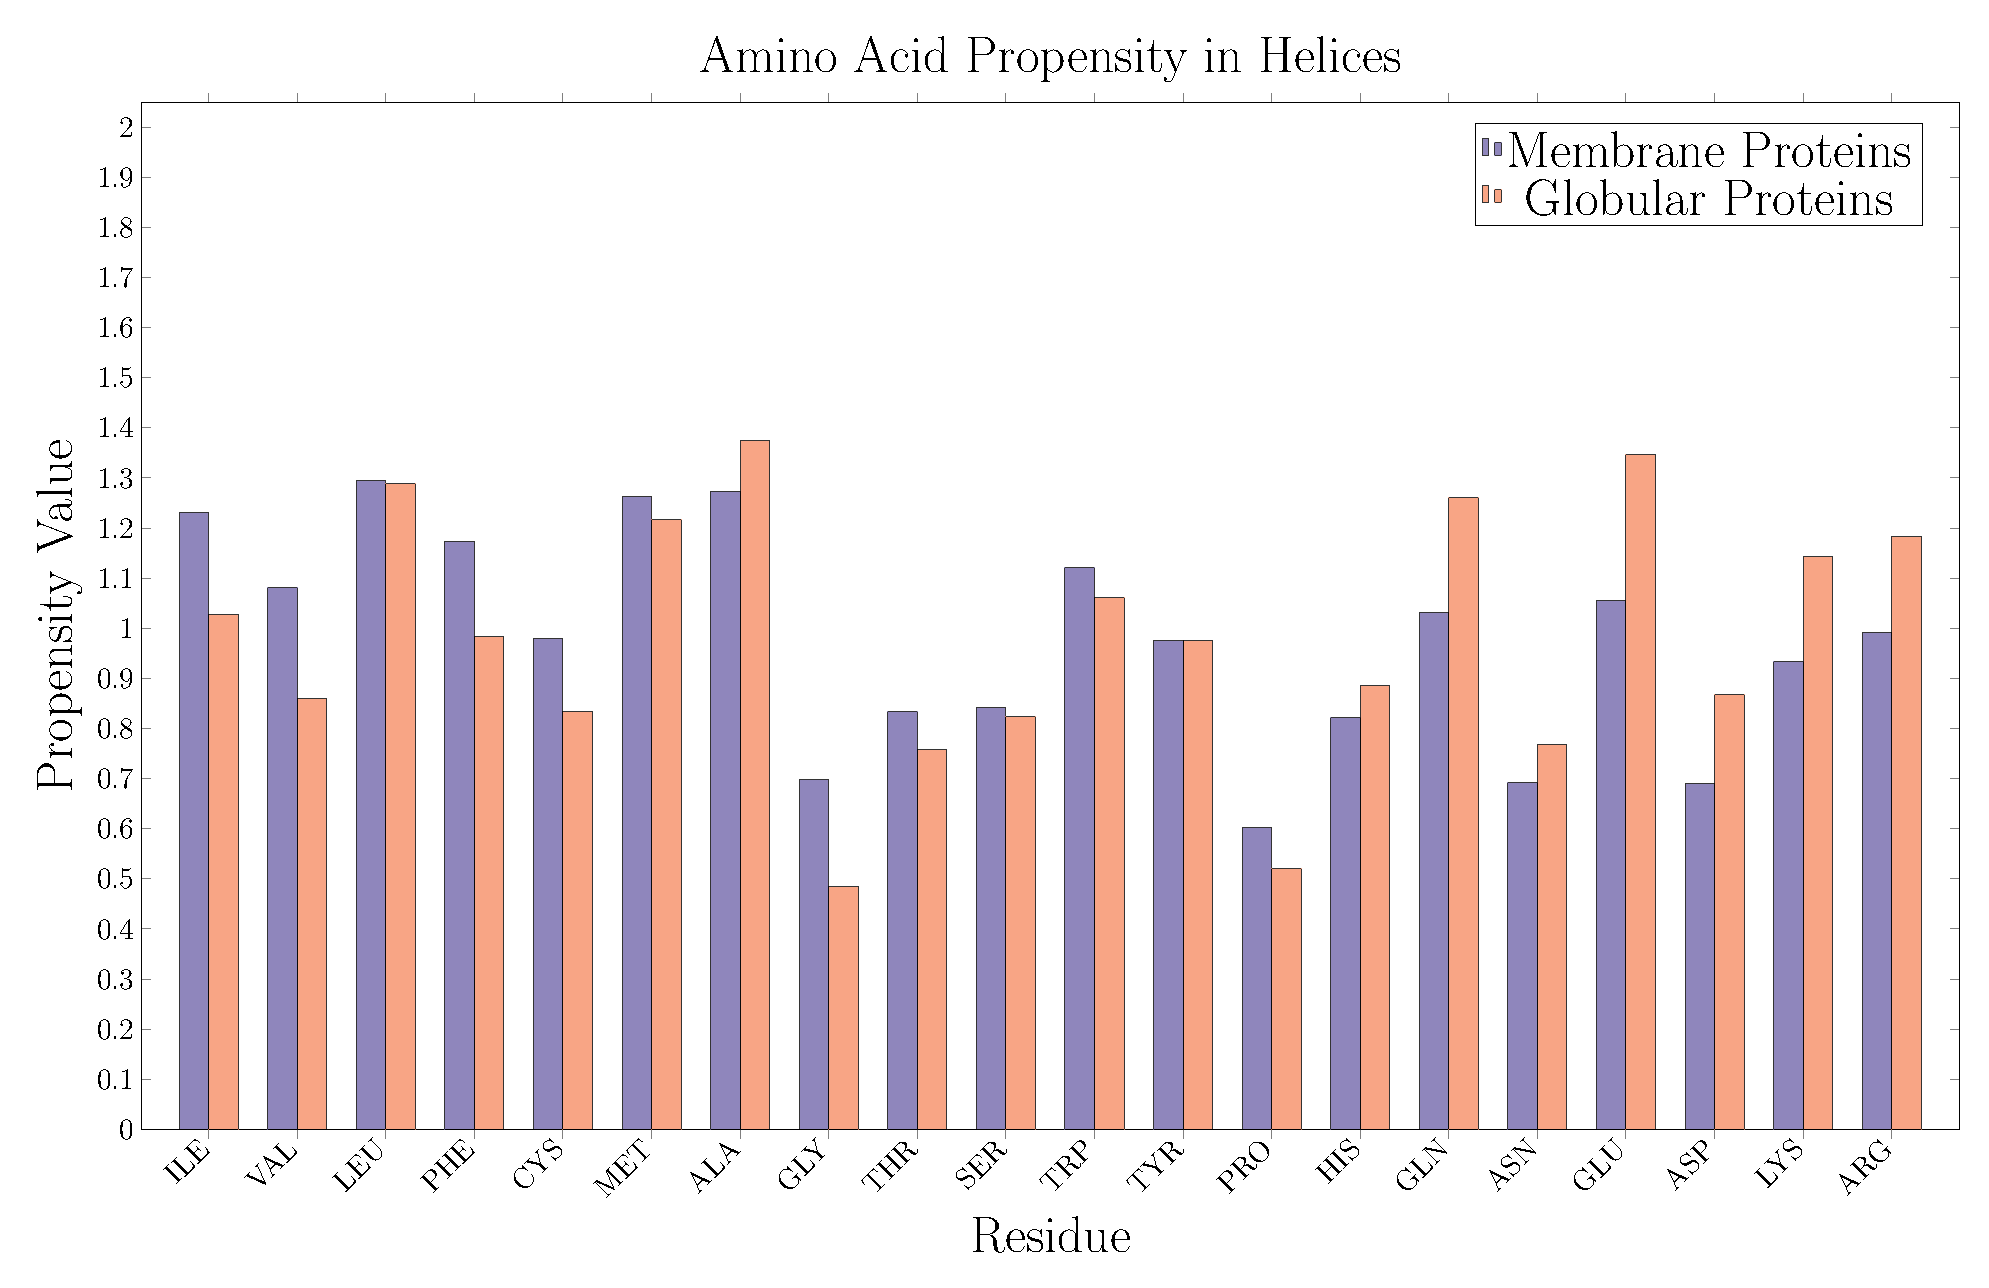
\includegraphics[width=0.025\textheight]{propensity_helices_r2dot8.pdf}};
			\node[align=center] at (25cm,5.cm) {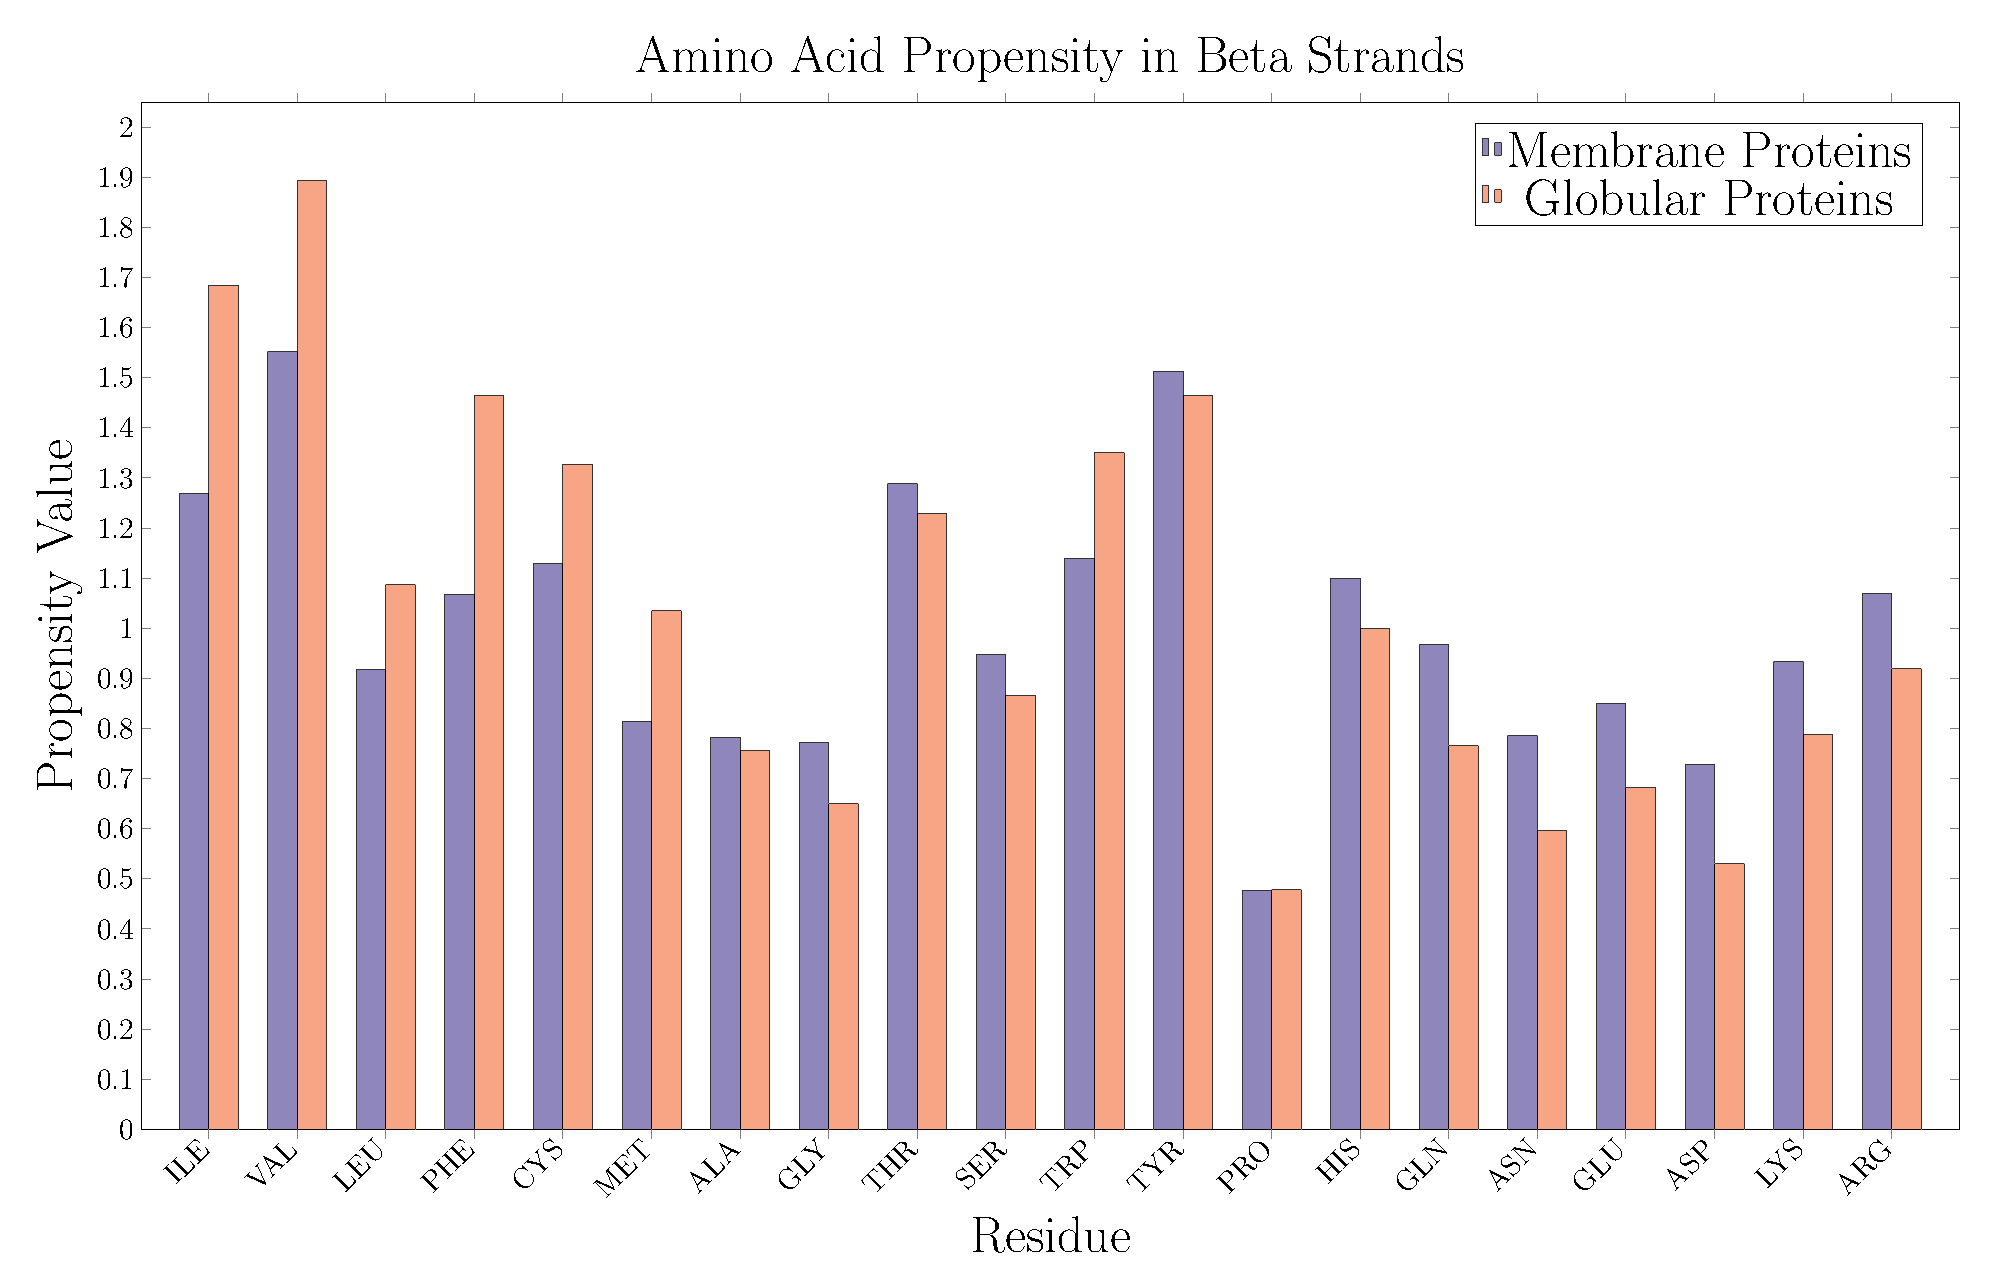
\includegraphics[width=0.025\textheight]{propensity_strands_r2dot8.pdf}};
			\node[align=center] at (10cm,-5.cm) {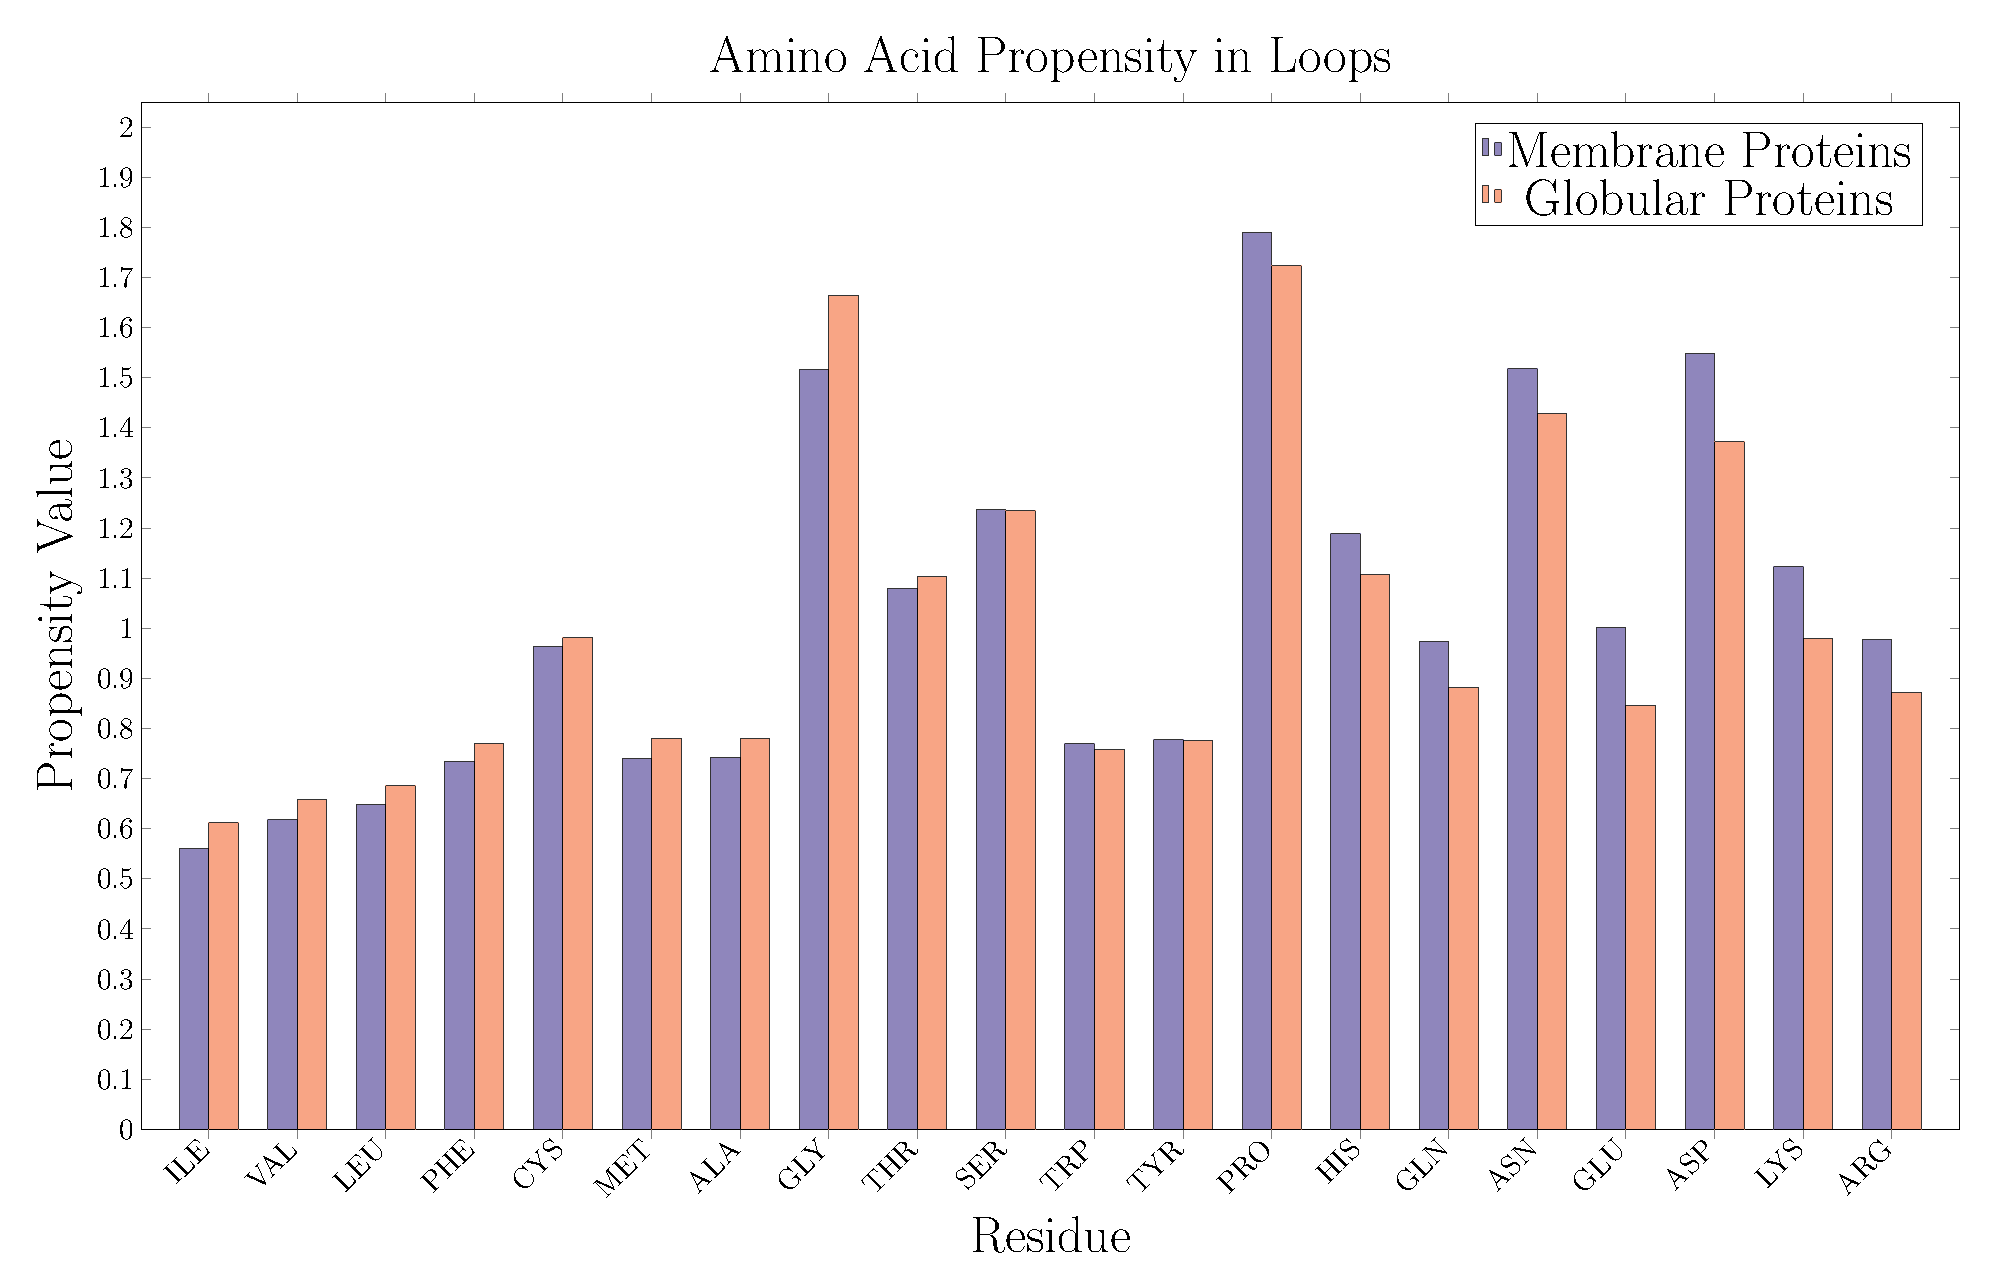
\includegraphics[width=0.025\textheight]{propensity_loops_r2dot8.pdf}};
			\node[align=center] at (25cm,-5cm) {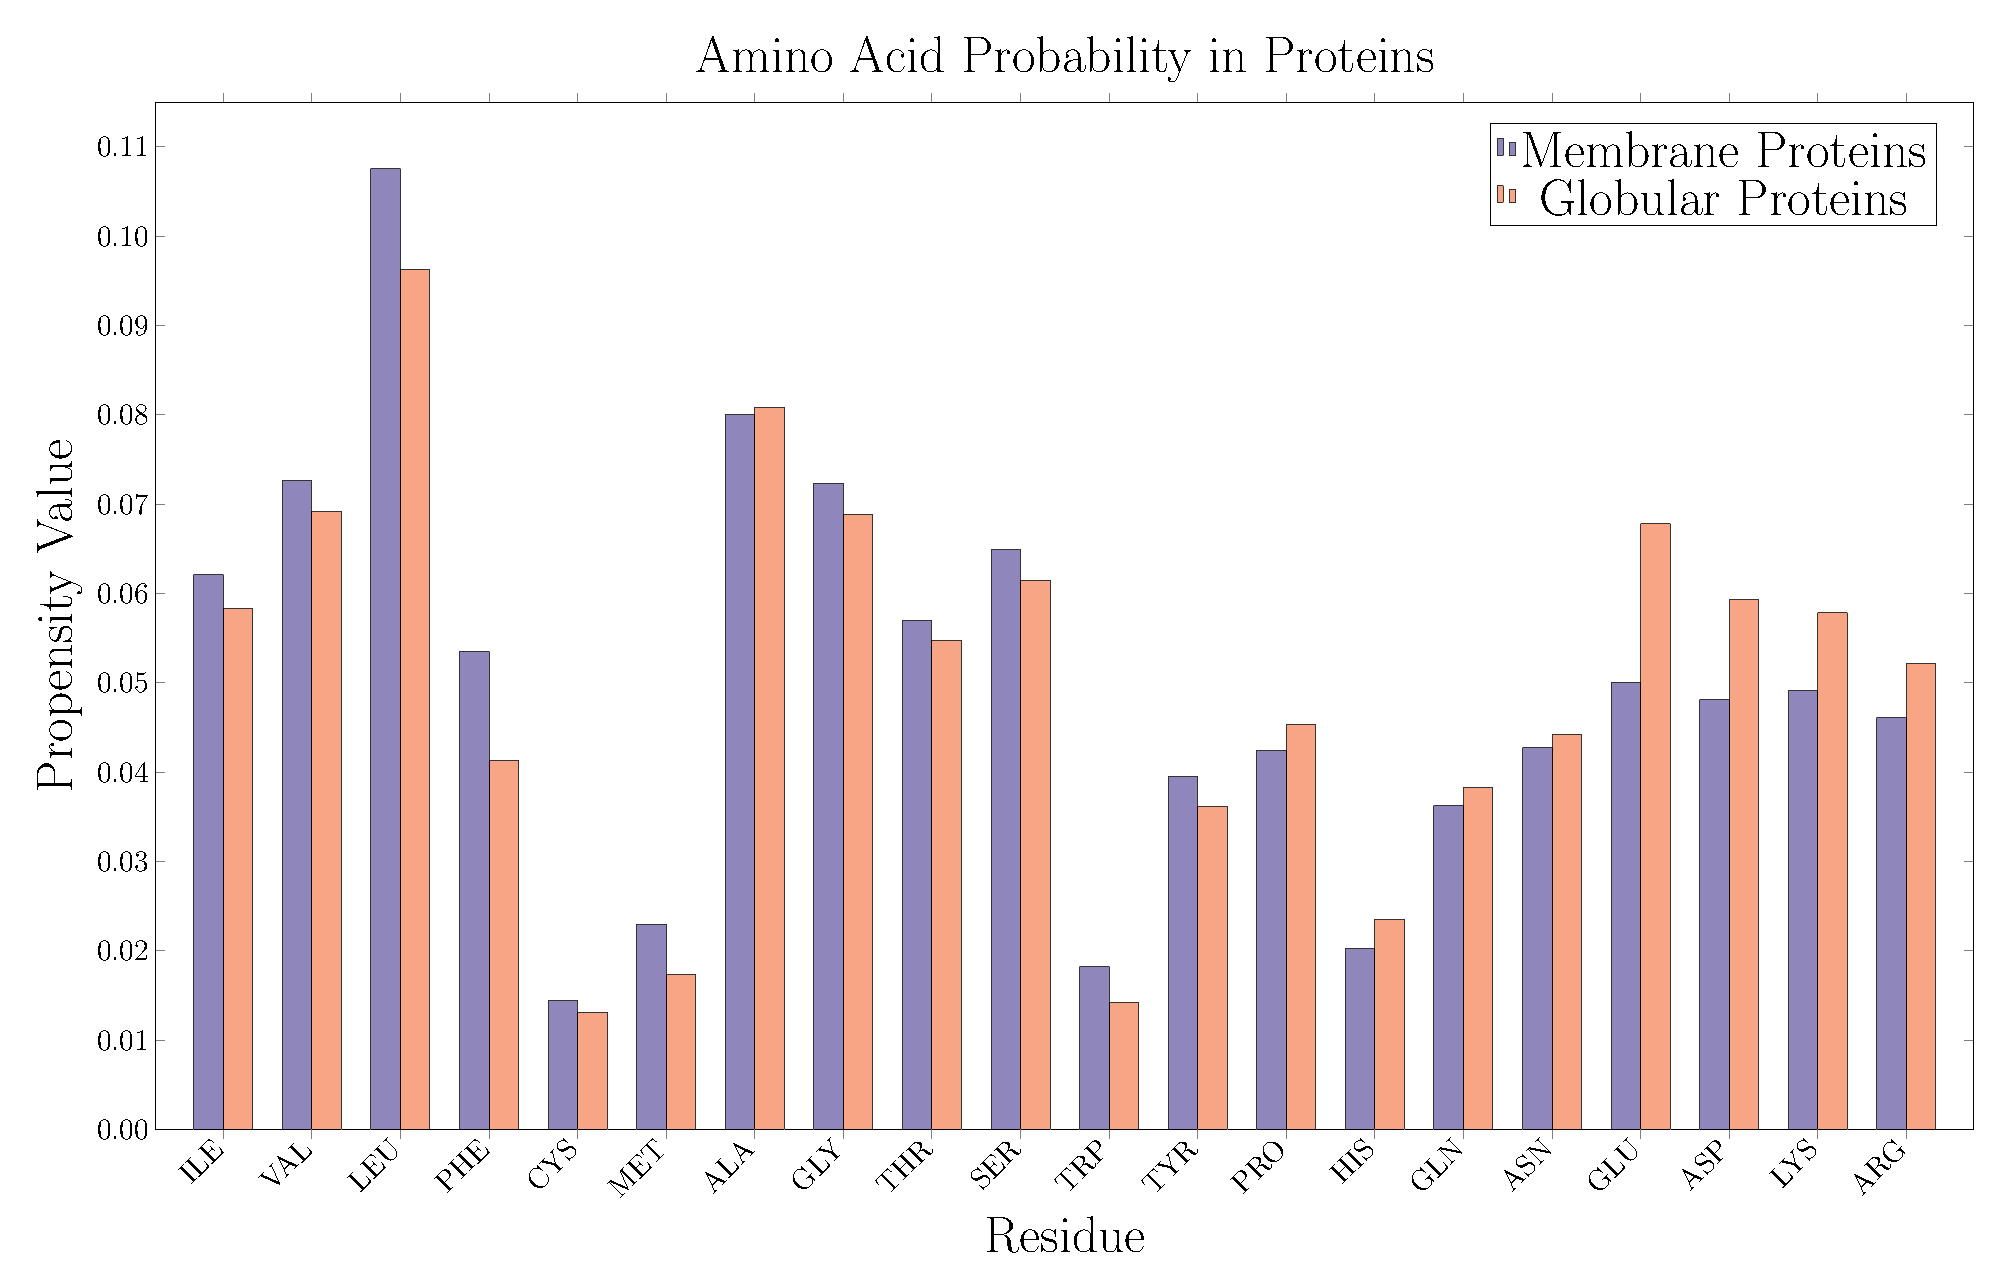
\includegraphics[width=0.025\textheight]{probability_aa_r2dot8.pdf}};
			
		\end{tikzpicture}
\end{document}  
